\documentclass[11pt,twocolumn]{article}

\usepackage[utf8]{inputenc}
\usepackage{amsmath}
\usepackage{amssymb}
\usepackage{parskip}
\usepackage{mathtools}
\usepackage{listings}
\usepackage{color}
\usepackage{hyperref}
\usepackage{graphicx}
\usepackage{caption}
\usepackage{subcaption}
\usepackage[noend,linesnumbered]{algorithm2e}
\usepackage{setspace} 
\DeclarePairedDelimiter\ceil{\lceil}{\rceil}
\DeclarePairedDelimiter\floor{\lfloor}{\rfloor}
\usepackage[left=1in,right=1in,top=1in,bottom=1in]{geometry}
\usepackage{amssymb}
\usepackage{dblfloatfix} % get tables to position at bottom of page
\usepackage{fixltx2e} % fix out of order figures
\newcommand{\footlabel}[2]{%
    \addtocounter{footnote}{1}%
    \footnotetext[\thefootnote]{%
        \addtocounter{footnote}{-1}%
        \refstepcounter{footnote}\label{#1}%
        #2%
    }%
    $^{\ref{#1}}$%
}

\newcommand{\footref}[1]{%
    $^{\ref{#1}}$%
}
\let\oldemptyset\emptyset
\let\emptyset\varnothing

\begin{document}

\title{CSE 221 Project Report}
\author{Jules Testard \quad Richard Park}
\maketitle

\section{Introduction}

\begin{table*}[t]
\centering
\begin{tabular}{| c | c |}
\hline
Jules Testard & Richard Park \\
\hline
 Procedure call overhead & Measurement overhead \\
System call overhead & Loop overhead \\
Task creation time overhead & Context switch time overhead \\
Entire Memory section & Entire Network section \\
Disk bandwidth & Network Disk Bandwidth \\
Disk Contention & File Cache Size \\
\hline
\end{tabular}
\caption{Workload}
\label{tab:workload}
\end{table*}

The goal of this project is to determine the performance characteristics of Richard's machine when running Ubuntu. We have made our experiments using C and assembly instructions without the help of external tools. The C compiler we have used is the gcc compiler (version 4.8.2). Optimization settings we have used for our compiler settings have varied across our measurements (more details in the paper). The workload for the project has been shared as shown in table [\ref{tab:workload}]. We estimate having spent each around 40 hours on the project, account for 80 hours total.

\section{Machine Description}

We are using a Lenovo Thinkpad X220 running the Ubuntu 12.04 operating system with the 3.5.0-54 kernel. The specs of the machine are described below. Some of the following information could be directly found through the system by reading /proc/cpuinfo. Some of this information could only be derived from online documentation. In all cases, the origin of the derivation of the characteristics is shown.

\subsection{Processor}
The machine possesses a Intel(R) Core(TM) i5-2520M processor. 

\begin{itemize}
    \item{Each core has a clock frequency of 2.5 GHz}
    \item{The core has a separate data and instruction L1 cache. Each cache is 2 x 32 KB.}
\item{The L2 cache size is 2 x 256 KB.}
\item{The L3 cache size is 3 MB.}
\item{The processor uses a 64 bit instruction set.}
\end{itemize}

\subsection{Buses}

The machine uses the Intel terminology for buses. Data transfer between the CPU to the memory is done through a 5 GT/s front side bus (FSB). The machine uses PCI Express 2.0 buses for I/O purposes.

\subsection{Memory}

The machine possesses two DDR3 4GB memory banks. Both banks use the memory bus mentioned earlier (FSB). The memory banks support but do not use error correcting codes (ECC). 

\subsection{Storage}

The machine uses a 256 GB Samsung 830 Solid State Drive. The max sequential
reads occur at 520 MB/s and the max sequential writes occur at 400 MB/s. The max random read speed is 75K IOPS and max random write speed 30K IOPS. 



\section{CPU Operations}

\subsection{Measurement Overhead}

In order to accurately measure execution time we implemented a timing
methodology that reads the hardware time-stamp counter before and after a
procedure (by procedure here we mean lines of C or assembly code we wish to
profile, not necessarily a procedure call).  The time-stemp is read immediately
before the procedure is called and again after the procedure exits. The two
output values correspond to the start and end times of the procedure being
executed. The initial time is subtracted from the final time to calculate the
number of cycles that have elapsed.

The implementation for reading the time-stamp makes use of the assembly
instructions CPUID, RDTSC, and RDTSCP. CPUID and RDTSCP are used to force
serialization of instructions so that instructions which are not part of the
code being instrumented do not pollute our measurements due to out-of-order
execution.\cite{intel}

We run the timing harness and procedure being timed in a loop of 10,000
iterations. The execution time is collected on each iteration of the loop. We
use the median execution time over all iterations as the final result in order
to reduce the influence that extreme values caused by context switches,
interrupts and other exceptional events have on our experiment. 

\subsubsection{Measuring time overhead} 

We estimate that the hardware overhead of reading the time-stamp registers and
calculating the elapsed time is 2 cycles. Since the time-stamp is implemented in
registers it would require 1 cycle to read the current time. 

We implemented the reading of the start and end time with inline assembly. The
code to read the start time and the code to read the end time each consists of
four assembly instructions. This includes the calls to CPUID which act as a
fence to force sequential execution of code.  Since the time-stamp register is
64-bits we retrieve the upper and lower 32-bits into two separate registers. We
reform the original 64-bit value by using a shift and bitwise or
operation.Finally,  The two 64-bit values are subtracted to produce the final
elapsed time in cycles. We estimate the software overhead to be 15 cycles.

The total overhead of our measuring mechanism is estimated to be 17 cycles.

In order to gain the most accurate measure of the timing overhead we disabled
additional cores and frequency scaling within the bios.

For computing the overhead of reading time, we ran the timing harness that was
previously described without any intervening code.  Our results show that the
overhead of reading time to be 40 cycles. 

Our results show that we underestimated the overhead of our timing mechanism. We
believe this is due to our assumption that the instructions CPUID and RDTSCP,
which is a serializing version of RDTSC, executes in a single cycle. We were
able to verify this by removing the CPUID calls and replacing RDTSCP with RDTSC.
The experiment without the serializing instructions showed that the overhead of
the timing mechanism was 22 cycles which is closer to our estimated result.

\subsubsection{Measuring loop overhead}

For the looping overhead,  we have to be careful that our looping procedure does
not get optimized out either by the compiler or the assembly interpreter. For
example, an empty loop would be quickly optimized with a constant propagation
compiler pass.  In order to ensure that no optimizations are performed,  we
disable compiler optimizations by using the "-o0" flag and implemented our
procedure under test using inline assembly.

The procedure under test is a loop, written in 5 lines of assembly code, that
runs for 10 iterations.  We estimate that a loop would not add any hardware
overhead. In terms of software overhead, we estimate that 5 additional cycles
will be required for each iteration of the loop. This number was arrived at by
examining the assembly code that implements the loop and assuming that each
instruction executes in a single cycle.

Our results show that our estimate of the loop overhead was very close to the
measured loop overhead of 4 cycles. The discrepency is the result of counting an
instruction that initializes the number of loops to perform by moving a
parameter into a register. This instruction does not participate in the actual
loop.

An interesting result that we discovered is that after several iterations of the
timing procedure (i.e. timing and loop of ten iterations) the loop overhead is
reduced to a single cycle. We suspect this is due to optimizations which are
occuring in the hardware in spite of disabling optimizations during compile
time.

\subsection{Procedure call overhead}

Here as well, we had to be careful about compiler optimizations. Again we used
the \texttt{rand()} function. The procedures we profile makes a unique call to
the rand() function and returns (and never uses any of its arguments). We create
eight such procedures (with 0 to 7 arguments).

Using our methodology, we measured the average time required for a single call
to the \texttt{rand()} function and each of our eight procedures (and compute
the difference). Measurements available soon.

\subsection{System call overhead}

\subsection{Task Creation Time}

In order to compare the execution time of a kernel thread and a process, we
setup a (slow) fibonacci function which would be the only thing the kernel
thread or process would execute.

We were able to profile kernel threads using our methodology. The procedure
between the two hardware counters simply creates a kernel thread which runs the
fibonacci function waits for that thread to complete. The average time spent by
the thread was 32264 cycles.

While kernel threads can be measured using our methodology, processes cannot be
created with a kernel module, since there is no fork or exec call in the linux
kernel API. As such for this task, we had to go out of kernel mode and write a
user program at the possible cost of loss of precision (however, this gave us
the opportunity to shut down compiler optimizations!). This time, we use a linux
\texttt{clone()} system call and had the child process execute the fibonacci
function. Measurements available soon.

\subsection{Context Switch Time} \subsubsection{Process Context Switch}
\subsubsection{Thread Context Switch}


\section{Memory Operations}

\subsection{RAM access time}

To measure RAM access time, we followed the methodology used in section 6.2 of the LmBench paper \cite{lmbench}. We created arrays of increasing sizes and iterated through them 1 000 000 times sequentially and would wrap around if we reached the end of the array. Each such array is created at the beginning of an experiment and freed at the end. Thus, it has only one name, \texttt{array}. The contents of the arrays are filled as follows :

\begin{lstlisting}
for (int i = 0; i < size; i++)
  pA[i] = &pA[stride+i];
char* p = pA[0];
\end{lstlisting}

This way, the array can be traverse using the statement \texttt{p = *p;} according to the stride. The size of the arrays created varies from 32KB ($2^{15}$) to 256MB ($2^{28}$). For each array size, strides 16,64,256 and 1024 are profiled. 

In terms hardware performance, our system has two 32kB L1 caches , 2 256kB L2 caches and 1 3MB L3 cache. From our vendor \cite{vendor}, we known that our cache lines are 128 bytes. In terms of software overhead, we attempted to minimize the effect of loop overhead by using loop enrolling on the \texttt{p = *p;} statement.

The result of our experiment is shown on figure \ref{fig:b2blatency}. The resulting graph is similar to the one found in the LmBench paper. The transition from L1 cache to L2 cache and L3 cache to main memory are clearly visible and present where expected. The transition from L2 cache to L3 cache isn't noticeable, however. We also notice that when the stride size becomes greater than the cache line of the hardware, the main memory latency is greatly increased.

\begin{figure}
 \centering
  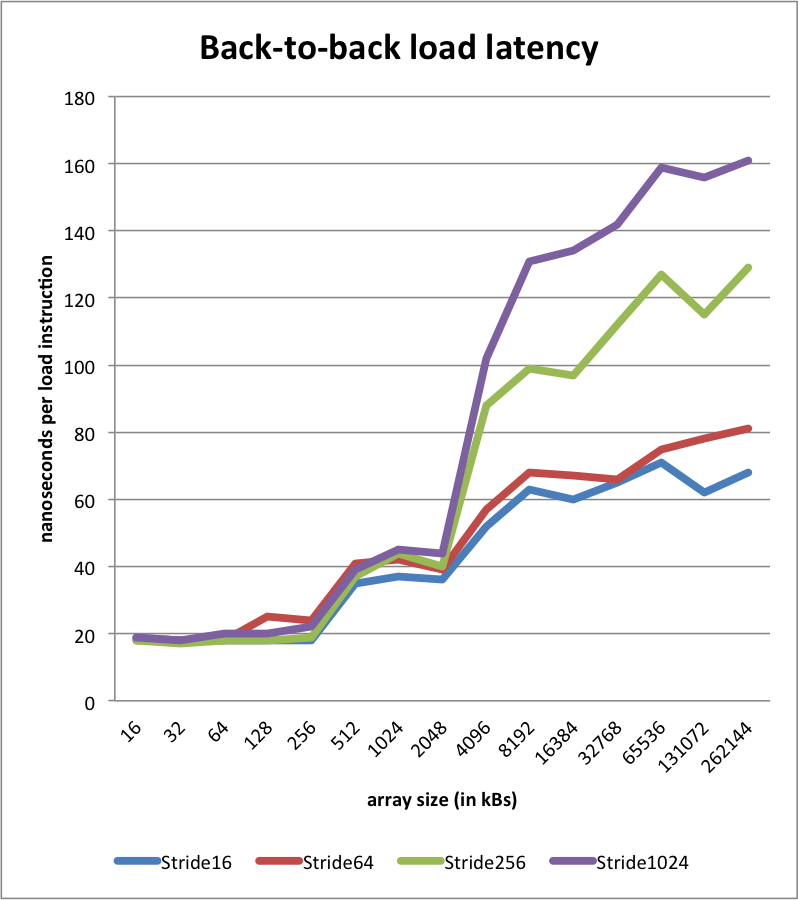
\includegraphics[width=0.5\textwidth]{image/backtobackload.png}
  \caption{Back To Back Load Latency}
 \label{fig:b2blatency}
\end{figure}

\subsection{RAM bandwidth}

To measure RAM bandwidth, we followed the methodology suggested by the LmBench paper. However, we used the \texttt{mempcy} function since the \texttt{bcopy} function used in the paper has been deprecated since.

\subsubsection{RAM read bandwith}

For the read bandwidth, we created two arrays (of type \texttt{char}), called \texttt{bigArrayR} (162MB) and \texttt{smallArray} (3MB). \texttt{bigArray} is filled with random data before the beginning of the profiling (using \texttt{rand()}). When profiling starts, the contents of \texttt{bigArrayR} are sequentially read into \texttt{smallArray} in chunks of 3MB using \texttt{memcpy}  (in an enrolled loop).

The small array has been chosen to be exactly of the size of our L3 cache. After being repeatedly written into, it is expected that it will fill the contents of the cache, and all reads from \texttt{bigArrayR} are expected to originate from RAM. In terms of hardware performance, according to our vendor \cite{lenovo}, our RAM has a 10GB/s copy bandwidth. In terms of software overhead, according to the LmBench paper, pure read represents only about one half to one third of the \texttt{memcpy} work. Therefore, we can expect read bandwidth to run at twice the speed of a \texttt{memcpy} procedure call.

We obtained a read bandwidth by multiplying by 2.5 the time taken for reading the entire \texttt{bigArrayR} (averaged over 5 runs). This gives us a RAM read bandwidth of 13.62 GB/secs.

\subsubsection{RAM write bandwidth}

For the write bandwidth, we keep \texttt{smallArray} and create a new empty array \texttt{bigArrayW} (162MB), left empty this time. When profiling starts, contents from \texttt{smallArray} are sequentially written into \texttt{bigArrayW} in chunks of 3MB using \texttt{memcpy} in an enrolled loop.

After being repeatedly read from, it is expected that the contents of \texttt{smallArray} will fill the L3 cache, and all writes to \text{BigArrayW} will be written to RAM. Hardware performance and software overhead remain the same.

We obtained a read bandwidth by multiplying by 2.5 the time taken for write to the entire \texttt{bigArrayW} (averaged over 5 runs). This gives us a RAM write bandwidth of 8.90 GB/secs. This confirms the 10GB/s RAM copy bandwidth advertised by our vendor. Notice that read bandwidth is slightly higher than write bandwidth. One possible reason for this is given in the LmBench paper: in some processors, \emph{write transaction turns into a read followed by a write to maintain cache consistency}.

\subsection{Page Fault Service Time}

To profile page faults, we have used a mechanism proper to the Linux operating system called \textbf{Cgroups}. Cgroups are "tags" which can be specified when running process and which indicate to the operating system that only a restricted set of resources (indicated in the Cgroup description) should be allocated to the process. For example, we have restricted the amount of RAM used by the process for this experiment to 75MB.

In the experiment, we proceed to allocate an array (called \texttt{mallocs}) of 150 strings, each 1MB long. In order to ensure that the memory is actually allocated, we fill these 1MB strings with actual data. The memory allocation is done sequentially (the string for \texttt{mallocs[0]} is constructed before the string for \texttt{mallocs[1]} and so on...).

\begin{figure}
 \centering
  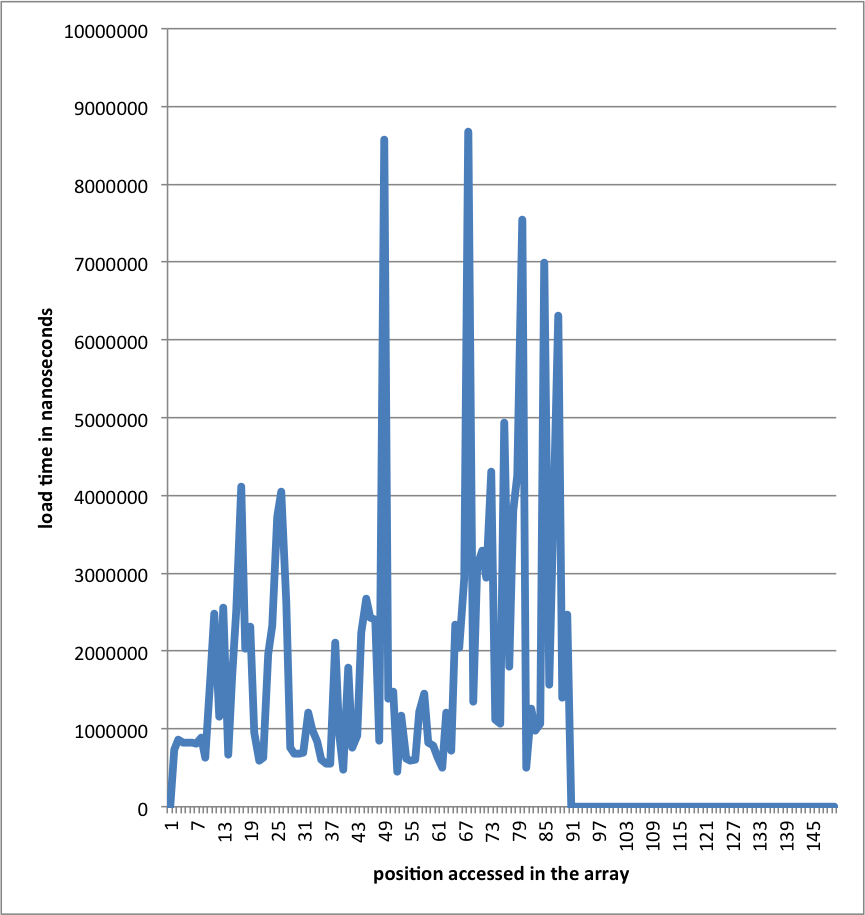
\includegraphics[width=0.5\textwidth]{image/pagefault.png}
  \caption{Page faults when accessing 150MB array}
 \label{fig:pagefault}
\end{figure}

Given the process can only 75MB of RAM, we can expect that at least half of the pages used by the \texttt{mallocs} array have been flushed to disk. Given data has been allocated sequentially, we can expect (according to the LRU rule), that these pages correspond to the first half of the array. The hardware performance of our SSD has been given by our vendor as a 750MB/sec read bandwidth. Software overhead is expected to be negligible in this experiment. However, in the context of a page fault, we can expect that after waiting for a while the OS might decide to do a context switch before coming back. Such context switch could occur while the process is waiting for a load instruction which is being profiled. As such, some fringe values in the experiment are to be expected as well.

These expectations are confirmed on figure ~\ref{fig:pagefault}. In this figure, we measure the time required to load each of the 1MB strings sequentially using \texttt{memcpy()} (we start by loading \texttt{mallocs[0]} and finish with \texttt{mallocs[149]}). We consider the 8-9 millisecond load times as the kind of fringe values we have to expect.
Given that the page size of our system is 4KB, 1MB corresponds to 256 pages. The median page load time for the first 90 MB is 1213/256 = 4.73  microseconds (which is consistent with the 750MB/sec bandwidth of our SSD). On the other hand, the average page load time for the last 60 MB is 0.8/256 = 0.00313  microseconds. This corresponds to a roughly 2000x increase when fetching pages from disk rather than main memory!



\section{Network}

The setup for our networking experiments consisted of our local machine
connected to a router and a remote machine connected to the same router over a
100Mbps Ethernet network. See the machine description section for a description
of the remote machine.

\subsection{Round Trip Time (RTT)}

\subsubsection{Estimation}

Our estimation of RTT for TCP is based upon an empirically derived lower bound.
The lower bound was determined by using the ping command to observe RTT for
ICMP packets sending and receiving 56 bytes of data to a remote host and
loopback. The overhead of TCP is greater than that of ICMP due to it being a
connected protocol that requires handshaking to establish a connection,
additional handshaking to close the connection, and a larger packet size.
Therefore, the RTT using TCP should be no faster than a ping to the same host. 

We observed that the average RTT for 1000 pings to the loopback were 0.033 and
to the remote machine 0.955ms. Transmitting 56 bytes of data via TCP requires
3.5 additional round trips because of connection overhead for the initial 3-way
handshake and 4-way termination which consists of 7 packets that each travel
one way.  We estimate the minimum RTT to loopback for an equivalent amount of
data (56 bytes) via TCP to be $$4.5 * 0.033\text{ms} = 0.145\text{ms}.$$  

The difference between the the ping time for loopback and to the remote machine
represent the overhead of packets crossing the physical network. Therefore we
estimate that the additional RTT for a single packet to the remote machine is
$0.955\text{ms} - 0.033\text{ms} = 0.922\text{ms}$. Clearly, the overhead of
crossing the physical network dominates the time to evaluate and send a packet
at its destination and source machine. It follows from our estimation of the
RTT to loopback that RTT to the remote machine for 56 bytes of data via TCP is
calculated as $$4.5 * 0.033\text{ms} + 4.5 * 0.922\text{ms} = 4.294\text{ms}.$$

\subsubsection{Methodology}

The program which runs on the local machine sets up a TCP connection and sends
a message to the remote machine. It waits for the message to return and then
tears down the connection. Each timing iteration begins immediately before
setup of the TCP connection and ends immediately after the connection is
closed. The program initializes a character array of 56 elements (i.e. 56
bytes) in order to perform an accurate comparison with ping which sends 56
bytes of payload per packet.  We use the sockets library to obtain a file
descriptor to a socket and then connect to the remote machine. We send to
socket 7 in order to be consistent with RFC 862 \cite{rfc862} which sets the
specification for an echo service. Once a connection is successful we send the
56 byte message and then perform a blocking read which will wait for the
message to return from the remote machine. After a message is recieved we close
the TCP connection and stop timing. If the bytes read does not equal the bytes
sent, the result is not recorded due to packets being dropped and the iteration
is repeated until successful.

In order to implement a simple echo service on the remote machine, we used the
ncat program with the following command: 
\begin{verbatim}
ncat -l 7 --keep-open -c 'cat'
\end{verbatim}
The arguments to the command instruct the program to listen on port 7 for
incoming tcp connections and echo the data by executing the cat program on the
incoming data. The keep open parameter instructs ncat to continue listening for
new connections once a remote connection closes.

\subsubsection{Results}

We used the timing methodology described earlier in this paper that reports the
number of cycles elapsed between the start and end. We convert the cycle count
to milliseconds as described in timing overhead section and present our results
in table~\ref{table:rtt-results}.

\begin{table*}[b]
\begin{tabular}{|c|c|c|c|}
\hline
RTT Local (cycles) & RTT Local (ms) & RTT Remote (cycles) & RTT Remote (ms) \\ \hline
3850916            & 1.572          & 30172312            & 12.315          \\ \hline
\end{tabular}
\caption{RTT experimental results}
\label{table:rtt-results}
\end{table*}

\subsubsection{Analysis and Discussion}

Our estimates for the remote case were off by a factor of 3 and an order of
magnitude in the case of loopback. We realize that in our estimates we did not
account for the fact that TCP would require an work done at an additonal layer
of the TCP/IP stack versus the ICMP packet. This is due to ICMP being a network 
layer protocol, the same as IP which encapsulates the ICMP packet, while TCP is 
a transport layer protocol. The evaluation/formation of the TCP packet at the
transport layer adds additional overhead that is missing in our estimate, but 
represented in the experimental results. This overhead would be present in the 
local and remote machine. The router that connects the two machines operates 
at the network layer and would not contribute additional overhead versus ICMP 
because it does not read TCP header information.

Comparing the local and remote results reveals that the overhead of transmitting
over a network dominates that of the OS overhead by an order of magnitude 
even for machines connected to the same LAN.

The network is rated at a maximum of 100Mbps. Our results show that we achieve in 
the local case: $$\frac{(56*8)}{0.00157} * 10^{-6} = 0.296\text{Mbps}$$
and in the remote case: $$\frac{(56*8)}{0.0123} * 10^{-6} = 0.0364\text{Mbps}.$$
This is far below the maximum performance that the hardware is capable of because of
 the software overheads that are required for reading and creating packet header information.
Ultimately, it is the size of our payload that contributes most to the discrepency 
in performance. The maximum transmission unit (MTU) for TCP is 1460 bytes, 
however we are sending data in 56 byte chunks. The next experiment in peak bandwidth 
will provide more reasonable results regarding the difference between ideal 
hardware performance and real world performance over TCP.

\subsection{Peak Bandwidth}

We use the data collected in the previous experiment to assist us in
deriving an estimate for peak bandwidth over TCP to a remote and local
connection. We determined in the previous experiment that in order to 
gain maximum throughput with TCP we would need each payload to be 
equivalent to the MTU. The difference in throughput should increase 
by a factor of $\frac{1460}{56} = 26.07$. We believe the OS overhead at the transport 
layer of reading and forming packets will also increase due to the larger payload, but 
this should have a negligable effect on our estimate due to the message buffer being 
initialized to the size of MTU in advance. With this information we estimate that 
peak bandwidth for the local case will be: $$0.297\text{Mbps} * 26.07 = 7.74\text{Mbps}$$
and for the remote case: $$0.0364\text{Mbps} * 26.07 = 0.949\text{Mbps}$$.

\subsubsection{Estimation}
\subsubsection{Methodology}
\subsubsection{Results}
\subsubsection{Analysis and Discussion}
\subsection{Connection Setup}
\subsubsection{Estimation}
\subsubsection{Methodology}
\subsubsection{Results}
\subsubsection{Analysis and Discussion}
\subsection{Connection Teardown}
\subsubsection{Estimation}
\subsubsection{Methodology}
\subsubsection{Results}
\subsubsection{Analysis and Discussion}




\section{File System}

\subsection{File Cache Size}

\subsubsection{Estimation}

Linux uses all available memory as a file cache, therefore the minimum size
file cache is 0MB if applications and kernel are using the entire memory. With this information we estimate that the maximum size file cache is the 
total size of memory minus the size of the linux kernel. To estimate the size of memory occupied by the kernel we clear the file cache by executing 
the following command:
\begin{verbatim}
echo 3 > /proc/sys/vm/drop_caches
\end{verbatim}
and then running the free program to report memory usage statistics. This shows that 4GB out of 8GB in memory are available to be used as a file cache.

\subsubsection{Methodology}

We implement a program that reads files of varying sizes and reports the read bandwith. For smaller file
sizes we expect the bandwidth to be high. Once the size of the file exceeds the size of the file cache,
we expect to see a drop in read performance. The file size at which read bandwidth drops should 
correspond with the file cache size.

The program obtains a file descriptor to the raw disk in read only mode with the file cache enabled. 
We read from the file descriptor one MB at a time until the desired file size is reached and at that 
point the lseek64() system call is invoked to return the read pointer to the beginning of disk. The process of reading from beginning of disk to the current file size repeats until a timeout signal is asserted.
We begin timing before the first call to read and end timing after a set period of time. We determined 
empirically that 5 seconds is sufficient to perform enough repititions of entire file reads for all 
file sizes tested.

\subsubsection{Results}

Our results are presented in figure~\ref{figure:cacheresult}.

\begin{figure}
    \centering
    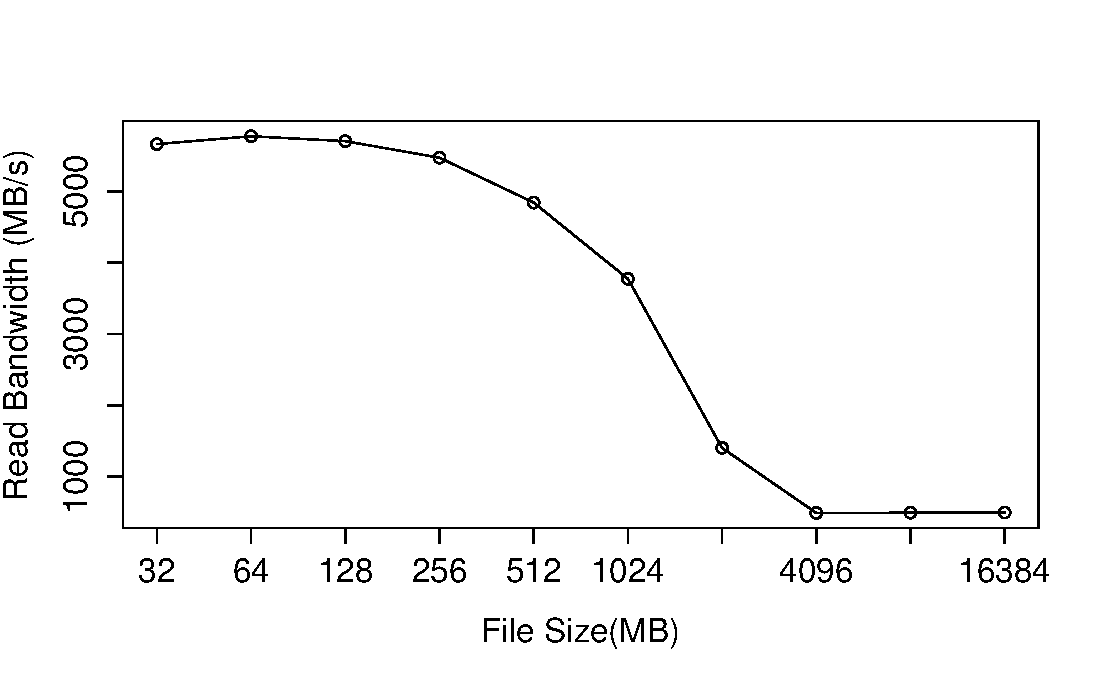
\includegraphics[width=0.5\textwidth]{cache-results.pdf}
    \caption{Experimental results for file cache size}
    \label{figure:cacheresult}
\end{figure}

\subsubsection{Analysis}

The results of our experiment show that for file read bandwidth exceeds the rated maximum bandwidth of the SSD (500MB/s) for file sizes greater than 4GB. This indicates that no file reads are cached because 
the file size is at least twice as large as the cache. According to our results we have over estimated the size of our file cache. The true size of the file cache appears to be between 512MB and 2GB where we 
see a corresponding decrease in the read bandwidth. 

\subsection{File Read Time}

In this section, we describe the time taken to read a file sequentially or randomly.

\subsubsection{Estimation}

Sequential access of a file is when we get the most out of the disk bandwidth. According to our vendor's specification, the maximum read throughput is 520MB/s. We are using a trick : we are not reading off a file that we have created. Rather, we are reading directly of from a disk partition, using a special file : \texttt{/dev/sda1}. In linux systems, \texttt{/dev/sda[x]} is the name of the special file representing disk partition \texttt{x}. There is no reason for a disk partition to be scattered across the disk (the way a user-generated file could be), therefore we can expect our disk access to be almost truly sequential (we still might have to fetch metadata on some other partition). As seen in class, we expect random access to be a lot slow than sequential access when accessing a file through disk. However, our machine uses a SSD, which are known to have much better seek times than traditional hard drives. 

\subsubsection{Methodology}

In order to ensure we are reading from disk and not from the file cache, we use the Linux flag \texttt{O\_DIRECT}. The \texttt{O\_DIRECT} flag can be specified when making the \texttt{open} system call. If used, it guarantees all read and write system calls on the opened file descriptor will fetch data from disk. We read from the \texttt{/dev/sda1} disk one MB at a time in a simple loop. We simulate different file sizes by setting a limit on the loop (called \texttt{total\_size}). When we reach the end of the loop we seek back to the beginning of the loop as follows : 

\begin{lstlisting}
if (total_read >= total_size) {
  retval = lseek64
     (fd, 0, SEEK_SET);
  total_read = 0;
  //...
\end{lstlisting}

where \texttt{total\_read} is the number of blocks read up to now in this iteration. To read blocks randomly, we also read directly from the disk partition. We use the \texttt{lseek} command which reads at an offset of a file descriptor, as follows:

\begin{lstlisting}
numblocks = SIZE_OF_FILE;
offset = (off64_t) numblocks *
  rand() / RAND_MAX;
retval = lseek64(fd, BLOCKSIZE 
  * offset, SEEK_SET);
\end{lstlisting}

where fd is the file seeked (in our case the disk partition), offset is the randomly chosen offset. \texttt{SEEK\_SET} is an option which tells the \texttt{lseek} command to start offsetting from the beginning of the file. Finally, we simulate files of varying size by changing the \texttt{numblocks} variable. To obtain the block size, we used a system command, \texttt{blockdev --getbsz /dev/sda1}; we found it was 4096. Notice we try to maximize bandwidth while reading truly randomly by seeking after each block read. If we read more than one block, than our read pattern would be partly sequential. If we read less, than we would not maximize our read bandwidth. Finally, in order to have good enough simulation we iterate continuously for 10 seconds and then measure the average time it takes to read one block into memory per millisecond.

\subsubsection{Results}

\begin{figure*}
 \centering
  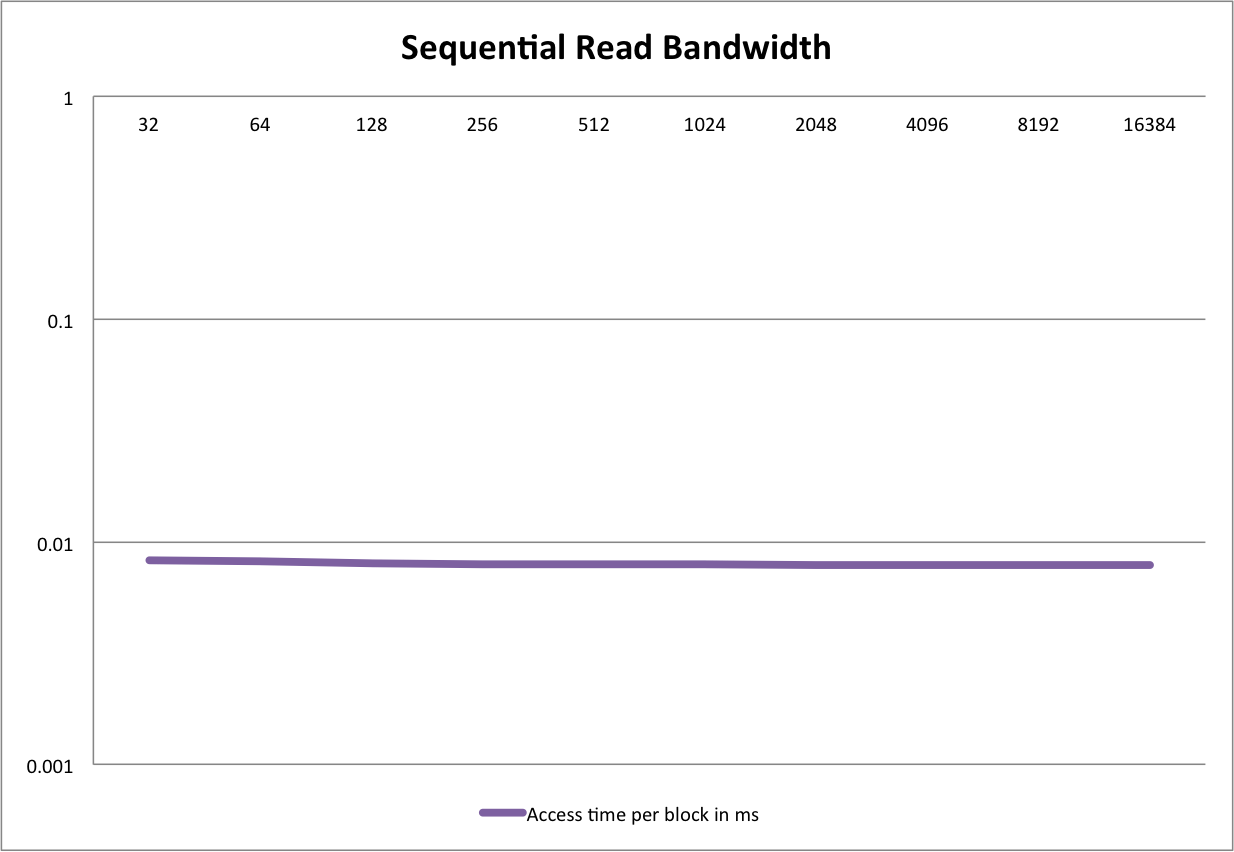
\includegraphics[width=0.85\textwidth]{image/sequential_read.png}
  \caption{Sequential Access Bandwidth}
 \label{fig:sequential}
\end{figure*}

\begin{figure*}
 \centering
  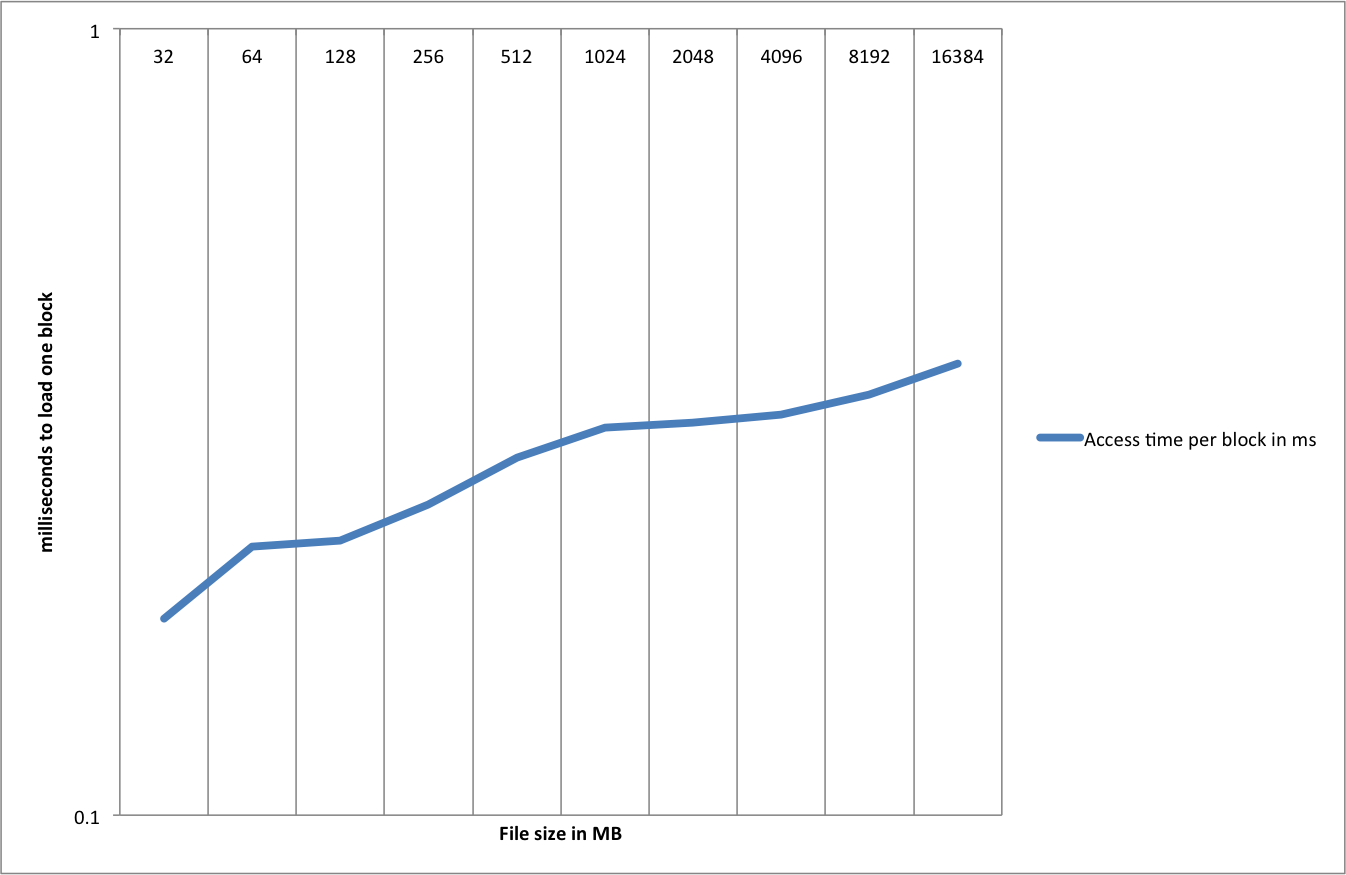
\includegraphics[width=0.85\textwidth]{image/random_read.png}
  \caption{Random Access Bandwidth}
 \label{fig:random}
\end{figure*}

\subsubsection{Analysis}

\subsection{Remote File Read Time}

\subsubsection{Estimation}

Our experiments used an exported file shared from an NFS version 3 server. NFS
version 3 uses TCP by default for data transport.  We estimate that the file
read bandwidth over NFS will be limited by the maximum throughput of the TCP
protocol. We will use the result from our peak bandwidth experiment to estimate 
that the file read bandwidth over NFS will be 16Mbps.

\subsubsection{Methodology}

We configure an NFS server on the same remote machine that was used in the Network bencmarking experiments and share a directory containing a 5GB file. The nfs share is mounted on our local machine and a 
modified version of the random access bandwidth experiment is performed. We modify the program for measuring the read bandwidth of random accesses so that O\_DIRECT flag is not used. This was required because 
it is not supported for reading NFS shares. Random access was chosen over sequential reads in order to limit the effect of the file cache upon our results.

\subsubsection{Results}

Our program outputs the results in MB per second as show in figure~\ref{figure:nsfresult}.

\begin{figure}
    \centering
    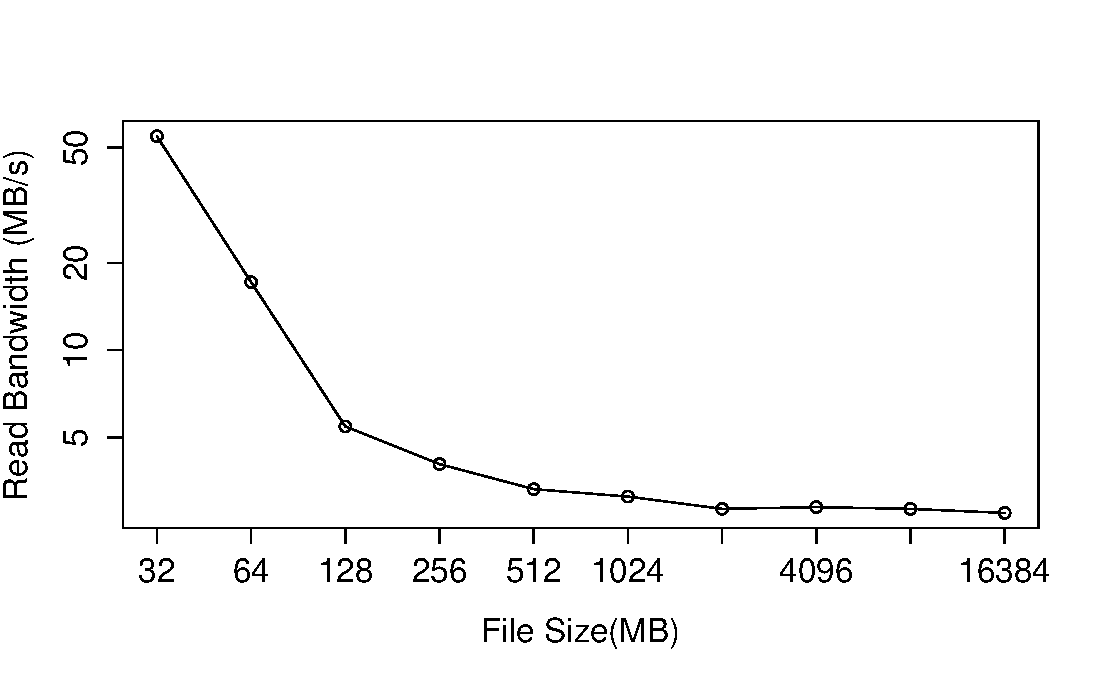
\includegraphics[width=0.5\textwidth]{nfsresults.pdf}
    \caption{log-log plot of experimental results for NFS read bandwidth}
    \label{figure:nfsresult}
\end{figure}

\subsubsection{Analysis}

The results show that read bandwidth is greater than our estimate for small
file sizes. This is due to data being accessed from the file cache.  The
experiment is run over the same period of time for each file size, therefore
smaller file sizes will have more opportunities for cache hits with random
access reads than larger file sizes because the overall working set is smaller.
The data shows that as file size increases, the read bandwidth approaches our
estimate that was based upon our previous experimental result of peak bandwidth
over TCP. The minimum read bandwidth is 2.7MB/s which is slightly better than
the peak bandwidth of TCP this is the expected result since the file cache was
not disabled due to reading files over NFS.

\subsection{Contention}

\subsubsection{Estimation}

\subsubsection{Methodology}

\subsubsection{Results}

\subsubsection{Results}

\begin{figure*}
 \centering
  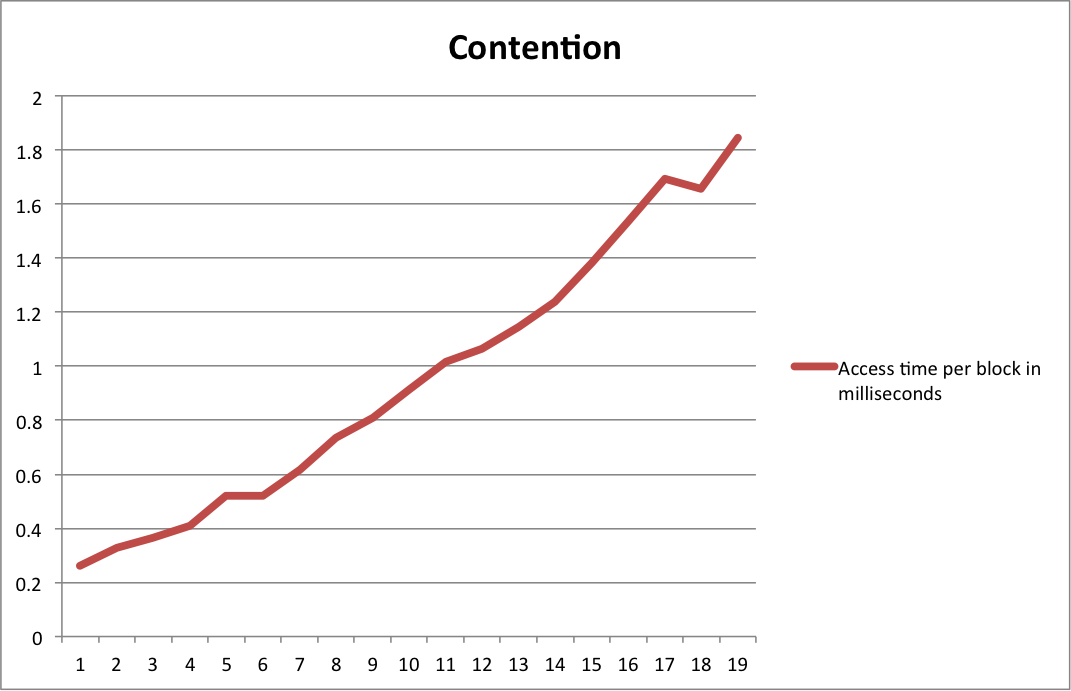
\includegraphics[width=0.85\textwidth]{image/contention.png}
  \caption{Sequential Access Bandwidth}
 \label{fig:contention}
\end{figure*}

\subsubsection{Analysis}


\begin{thebibliography}{9}
\bibitem{intel}
    \url{http://www.intel.com/content/dam/www/public/us/en/documents/white-papers/ia-32-ia-64-benchmark-code-execution-paper.pdf}
\bibitem{rfc862}
    \url{http://tools.ietf.org/html/rfc862}
\bibitem{lmbench}
    lmbench: Portable Tools for Performance Analysis. McVoy and Staelin. Proceedings of Usenix 1996
\end{thebibliography}
\end{document}
